% =====================================================================================================
%  ECONOMIC EVALUATION: LIQUIDITY-PROVISION BACKTEST -- paste-in blocks for manuscript.tex
%
%  Setup (once):
%   * copy  paper/generated/*.tex  into a folder  lp/  of the Overleaf project, and
%   * copy  figures/lp_*.png       into the project's  figures/  folder;
%   * add   \input{lp/lp_numbers}  to the preamble (after \usepackage lines).
%  All model-dependent numbers in the text are macros (\lp...) defined in lp/lp_numbers.tex, and the
%  tables are \input from lp/. After re-running  backtest.py, figures.py, paper_tables.py  re-copy both
%  folders; paper_tables.py prints CLAIM OK / CLAIM FAILS for every qualitative statement made below.
%  Bibliography: only keys already in updated.bib (Milionis2022, uniswap_whitepaper).
% =====================================================================================================


% -----------------------------------------------------------------------------------------------------
% [A] ABSTRACT -- insert after "... with statistically significant gains."
% -----------------------------------------------------------------------------------------------------
In a liquidity-provision backtest on the same pool, setting a vault's range from the forecast intervals
raises its risk-adjusted return relative to a Gamma-style vault, and pausing repositioning during
early-warning alerts more than halves its losses around depeg events; together, the two models reduce the
vault's maximum drawdown by \lpFcKvsGammaMaxDDCut\%.


% -----------------------------------------------------------------------------------------------------
% [B] HIGHLIGHTS -- add as a fourth item
% -----------------------------------------------------------------------------------------------------
\item Forecast ranges and early-warning pauses cut LP vault drawdowns in a backtest.


% -----------------------------------------------------------------------------------------------------
% [C1] INTRODUCTION -- new paragraph after the paragraph ending
%      "... while the forecaster characterizes its direction and severity."
% -----------------------------------------------------------------------------------------------------
Detection rates and scoring rules do not by themselves show that the models are economically useful,
particularly with few held-out events. We therefore evaluate the framework in the decision problem most
exposed to the pool's depeg risk: providing liquidity to it. A liquidity provider earns swap fees but loses
to arbitrageurs whenever the price moves, a cost measured by loss-versus-rebalancing (LVR)
\citep{Milionis2022}, and automated vaults that recentre a narrow range on the price amplify that cost
during depegs. In a backtest against a Gamma-style vault, each model has one role. The forecaster sizes the
range: using its predictive interval raises the vault's net profit and Sharpe ratio and reduces its
repositioning costs and daily tail losses. The classifier pauses repositioning during its alerts: this
cuts the LVR incurred around depeg events by \lpFcKEvLVRCut\% and the drawdowns within them by
\lpFcKEventDDCut\%, more than a price trigger at the same threshold or randomly timed pauses achieve. The
pause gives up part of the high fee income of depeg periods, so it acts as insurance rather than as a source
of return. A stress scenario based on the March 2023 USDC depeg, in which vaults that keep repositioning lose
20--30\% of their capital, illustrates the losses it protects against.

% [C2] INTRODUCTION -- replace the roadmap sentence
%      "Section \ref{sec:results} reports the empirical results, and Section \ref{sec:conclusion} concludes."
Section~\ref{sec:results} reports the empirical results, including the economic evaluation in
Section~\ref{sec:lp_results}, and Section~\ref{sec:conclusion} concludes.


% -----------------------------------------------------------------------------------------------------
% [D] METHODOLOGY -- new subsection at the end of Section 3, immediately before
%     "\section{Results}\label{sec:results}"
% -----------------------------------------------------------------------------------------------------
\subsection{Economic evaluation: a liquidity-provision backtest}\label{sec:lp_method}

We evaluate both models in the decision problem most exposed to the pool's depeg risk: providing liquidity
to it. A liquidity provider (LP) runs an automated vault in the USDC--USDT 0.01\% pool, like the Gamma vaults
that manage Uniswap V3 positions for their depositors. Every hour the vault decides the price range in which
its capital is deployed. A narrow range earns a larger share of swap fees, but the vault must reposition it
more often, paying gas and swap costs, and every price move inside the range is exploited by arbitrageurs
\citep{Milionis2022}. In a depeg, a vault that keeps recentring on the moving price repeatedly sells the
appreciating token and buys the depreciating one.

\paragraph{Position value, fees and loss-versus-rebalancing.} Let $P_k$ be the pool price of USDC in USDT at
the end of hour $k$. A position with liquidity $L$ on $[p_a,p_b]$ holds
$x(P)=L\big(1/\sqrt{\bar P}-1/\sqrt{p_b}\big)$ USDC and $y(P)=L\big(\sqrt{\bar P}-\sqrt{p_a}\big)$ USDT, with
$\bar P=\min\{\max\{P,p_a\},p_b\}$ and value $V(P)=x(P)P+y(P)$ \citep{uniswap_whitepaper}. Its fee income in
hour $k$ is
\begin{equation}
f_k=F_k\,\omega_k\,\frac{L}{L^{\mathrm{act}}_k+L},
\end{equation}
where $F_k$ is the pool's fee revenue, $L^{\mathrm{act}}_k$ its active liquidity and $\omega_k$ the share of
the hour's high--low price interval inside the range. The benchmark is the \emph{rebalancing portfolio} of
\citet{Milionis2022}: it holds the same USDC inventory as the position at the start of each hour and trades
at market prices. The position's loss relative to it,
\begin{equation}
\mathrm{LVR}_k=V(P_k)-V(P_{k-1})-x(P_{k-1})\,(P_k-P_{k-1})\le 0,
\end{equation}
is the price the LP pays to arbitrageurs, and the vault's net profit relative to the rebalancing portfolio is
\begin{equation}
\Pi_k=f_k+\mathrm{LVR}_k-c_k,
\end{equation}
where $c_k$ is the cost of repositioning: \$10 of gas per withdrawal and deposit, and the pool fee plus
0.5\,bp of slippage on the swap that restores the inventory required by the new range. The vault's value
satisfies $V_T-V_0=\sum_k\Pi_k+\sum_k X_{k-1}(P_k-P_{k-1})$, where $X$ is its total USDC holding; the second
term is the exposure to the USDC/USDT price, which the rebalancing portfolio shares, so $\Pi$ isolates the
consequences of the LP's decisions. All results are for a \$1M vault, in basis points of its capital.

\paragraph{Vaults.} Two standard vaults serve as benchmarks: a static range of $\pm5$ ticks (about
$\pm5$\,bp) around parity, never repositioned, and a Gamma-style vault that recentres a $\pm2$-tick range on
the current price whenever the price leaves it. The $\pm2$-tick width is the best recentring width both
before and during the holdout. Each model then has a single role, with no parameter tuned on the holdout.
\begin{itemize}
  \item \emph{Forecaster: range sizing.} The range is the forecaster's 10\%--90\% predictive interval, taken
        as the union of the intervals for the next six hours and extended to contain the current price, so it
        widens when uncertainty rises and leans towards the side where the forecast distribution places more
        mass. The vault repositions when the price leaves the range or when the target width becomes more than
        twice, or less than a third of, the current width.
  \item \emph{Classifier: pause during alerts.} During an alert episode, defined by the operating cutoff
        and 12-hour quiet reset of Section~\ref{sec:holdout_results}, the vault keeps its position and does
        not reposition. A position left in place leaves the range as the price moves away and then stops
        incurring LVR, instead of being recentred on the moving price. The classifier is used at the 15\,bp
        threshold for which it is trained.
\end{itemize}
The two-model vault uses the forecaster's ranges and pauses during the classifier's alerts. The same pause
is applied to the Gamma-style vault to isolate the classifier's contribution.

\paragraph{Controls.} Three controls separate the information in the classifier from the act of pausing. A
\emph{price trigger} pauses the vault while $|d_k|\ge15$\,bp, with the same quiet reset; it acts on the
events the classifier is trained to anticipate, but only once they have started. An \emph{oracle} pauses the
vault from 24 hours before each event. \emph{Placebo} schedules place the classifier's \lpEpisodes{} alert
episodes, with their durations, at \lpNPlacebo{} random sets of dates. Decisions are taken at the end of hour
$k$ for hour $k+1$; price rules use $P_k$, while model outputs are used with a one-hour data lag.

\paragraph{Performance and risk measures.} We report fee income, LVR, costs and net profit (annualised
$\sum_k\Pi_k$), the Sharpe ratio of daily and the Sortino ratio of hourly $\Pi$, the maximum drawdown of
cumulative $\Pi$, the worst day, and the 5\% conditional value-at-risk (CVaR) of daily $\Pi$. Because the
classifier targets rare events, we also measure risk where it materialises: the \emph{event drawdown} is
the sum, over the 15\,bp events, of the largest drawdown of cumulative $\Pi$ between 24 hours before and
48 hours after each event.

\paragraph{Samples.} The main sample is the common holdout coverage of both models, from \lpHoldoutStart{}
to \lpHoldoutEnd, with \lpNEvents{} events. As an out-of-sample check we use the classifier's 2024
cross-validation folds. The pool's subgraph records no fees before 19 March 2024, so this sample starts on
20 March 2024 and contains \lpYNEvents{} events; the neural forecasts cover only the holdout, so a rolling
empirical forecaster (the trailing 30-day distribution of $h$-hour price changes) stands in for them.


% -----------------------------------------------------------------------------------------------------
% [E] RESULTS -- new subsection at the end of Section 4, after Figure \ref{fig:stress_calm_ablation} and
%     immediately before "\section{Conclusion and Perspectives}"
% -----------------------------------------------------------------------------------------------------
\subsection{Economic evaluation}\label{sec:lp_results}

Table~\ref{tab:lp_main} reports the backtest over the holdout, and Figure~\ref{fig:lp_drawdowns} shows the
drawdowns over time. We discuss the benchmarks first, then the contribution of each model in turn.

\input{lp/tab_lp_main}

\begin{figure}[pos=!htbp,align=\centering]
    \centering
    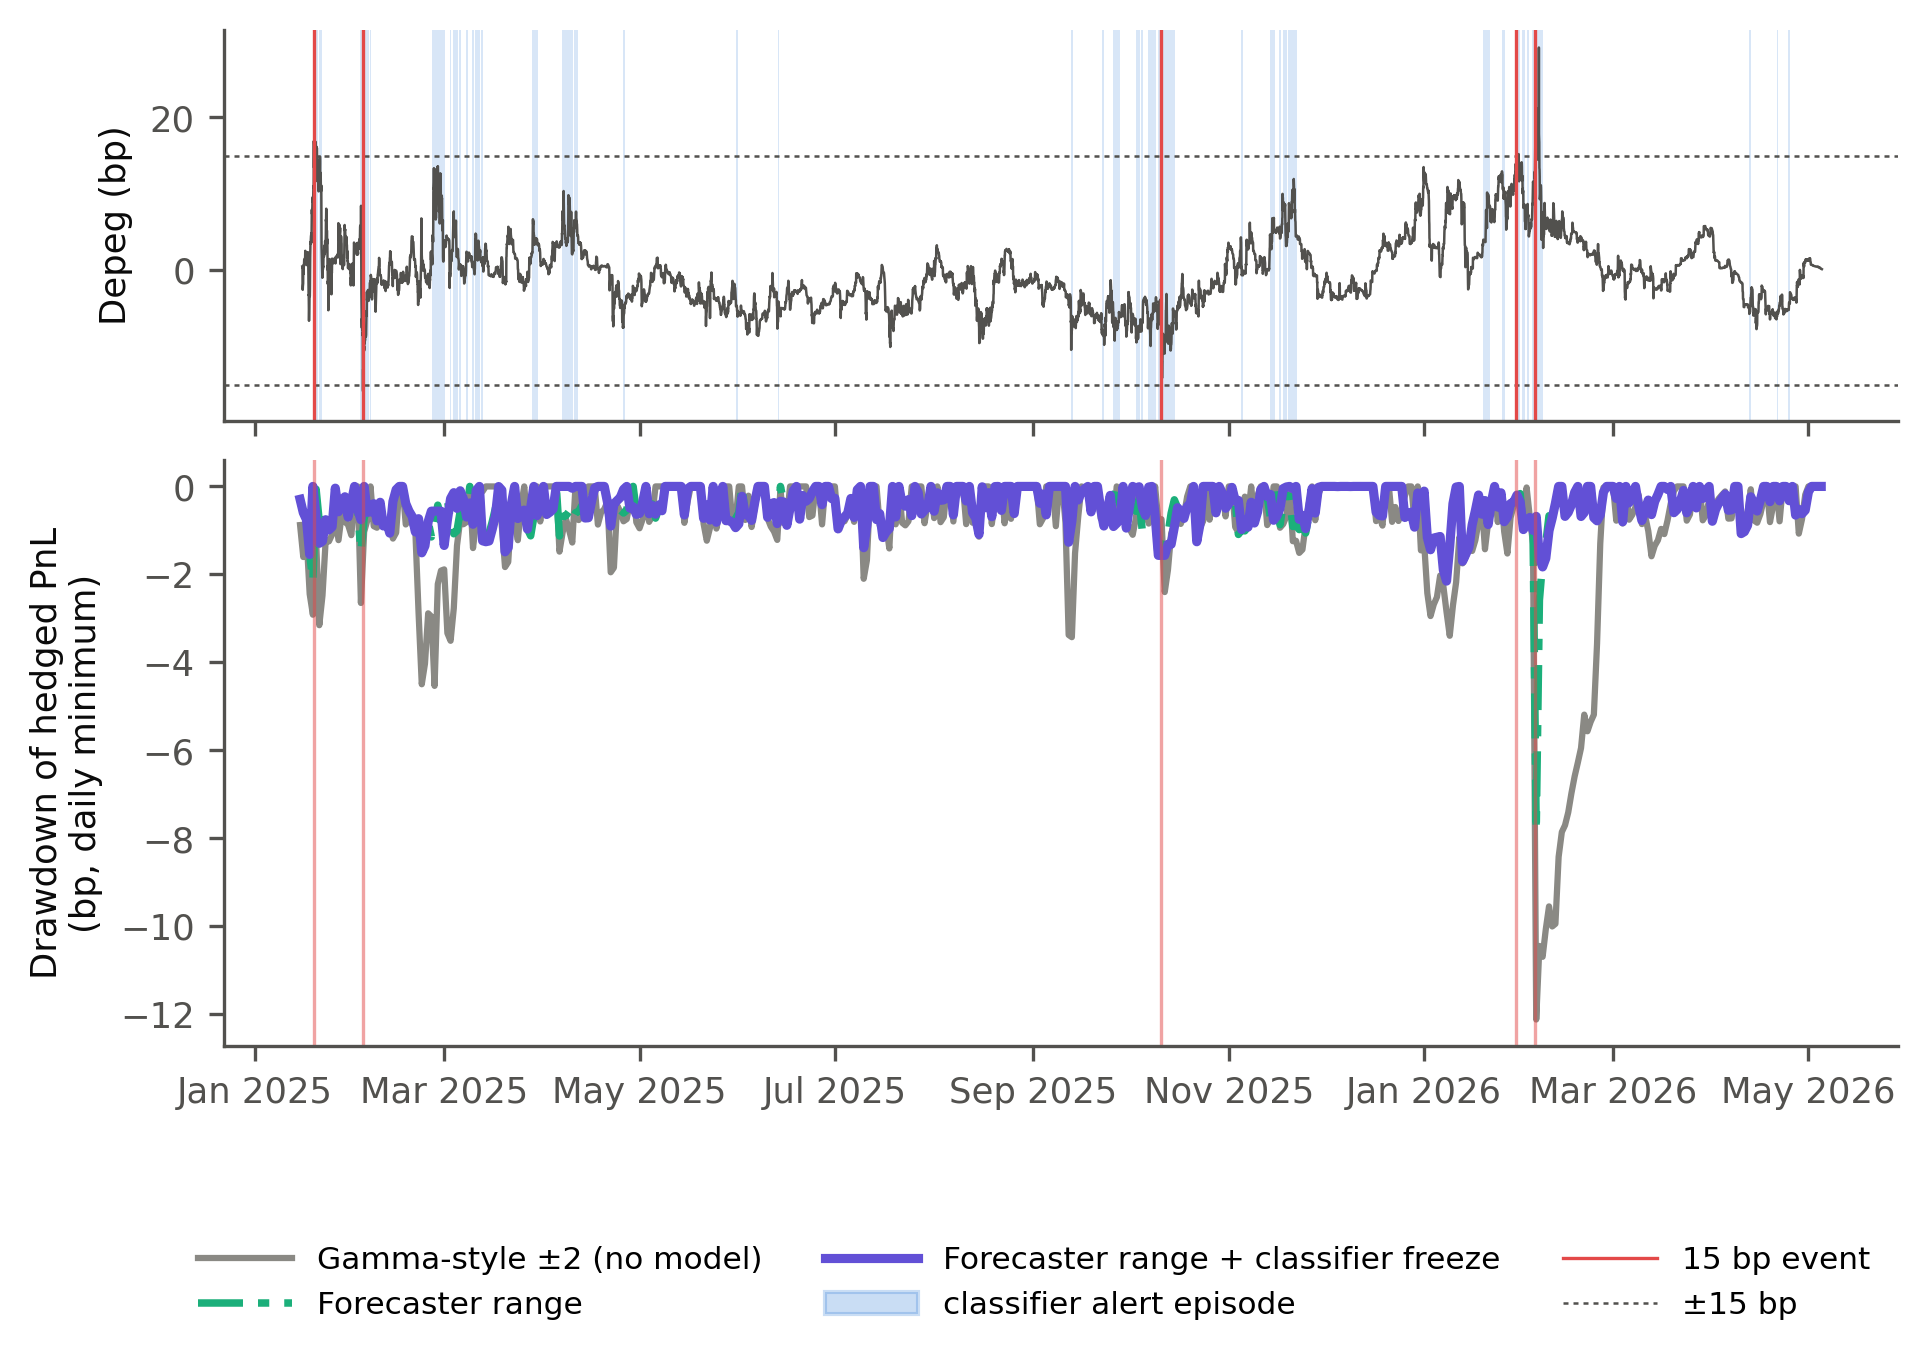
\includegraphics[width=\linewidth]{figures/lp_drawdowns.png}
    \caption{Top: pool depeg, classifier alert episodes and 15\,bp events over the holdout. Bottom: drawdown
    of the net profit of the Gamma-style vault, the vault with forecaster ranges, and the two-model vault,
    which also pauses during the classifier's alerts (daily minimum).
    \href{https://github.com/QuantLet/onchain-insights/tree/main/14.\%20LP\%20vault\%20backtest}{\includegraphics[height=0.6\baselineskip]{figures/Quantlet LOGO.png}}}
    \label{fig:lp_drawdowns}
\end{figure}

\paragraph{Benchmarks.} The static range is almost riskless but earns only \lpStaticNet\,bp per year, because
the price spends much of its time away from parity. The Gamma-style vault keeps its capital in the active
range and earns \lpGammaNet\,bp per year, but at a cost: it repositions \lpGammaRepo{} times a month, its
LVR and costs absorb half of its fee income, and its risk is concentrated in the depeg events. Its maximum
drawdown (\lpGammaMaxDD\,bp) and worst day (\lpGammaWorstDay\,bp) both occur in the event of
4 February 2026, when the pool price reached \lpMaxDepeg\,bp.

\paragraph{The forecaster sizes the range.} Replacing the fixed $\pm2$-tick range with the forecaster's
interval raises net profit by \lpFcNetGain\,bp per year, to \lpFcNet\,bp, and the Sharpe ratio from
\lpGammaSharpe{} to \lpFcSharpe. The interval widens when the forecast uncertainty rises, which lowers the
vault's repositioning costs from \lpGammaCosts{} to \lpFcCosts\,bp per year; its worst day improves from \lpGammaWorstDay{} to \lpFcWorstDay\,bp and its daily CVaR from \lpGammaCVaR{}
to \lpFcCVaR\,bp. Figure~\ref{fig:lp_fees_lvr} decomposes these gains: within the event windows, the
forecaster range reduces LVR by \lpFcEvLVRCut\% and costs from \lpGammaEvCosts{} to \lpFcEvCosts\,bp while
keeping most of the fee income. Sizing alone does not protect against a sustained depeg, however: the range
is still repositioned as the price keeps moving, and the vault's maximum drawdown (\lpFcMaxDD\,bp) again
occurs in the largest event. Asymmetric intervals outperform symmetric ranges of the same width centred on
the median forecast with every forecaster (Table~\ref{tab:lp_forecasters}).

\begin{figure}[pos=!htbp,align=\centering]
    \centering
    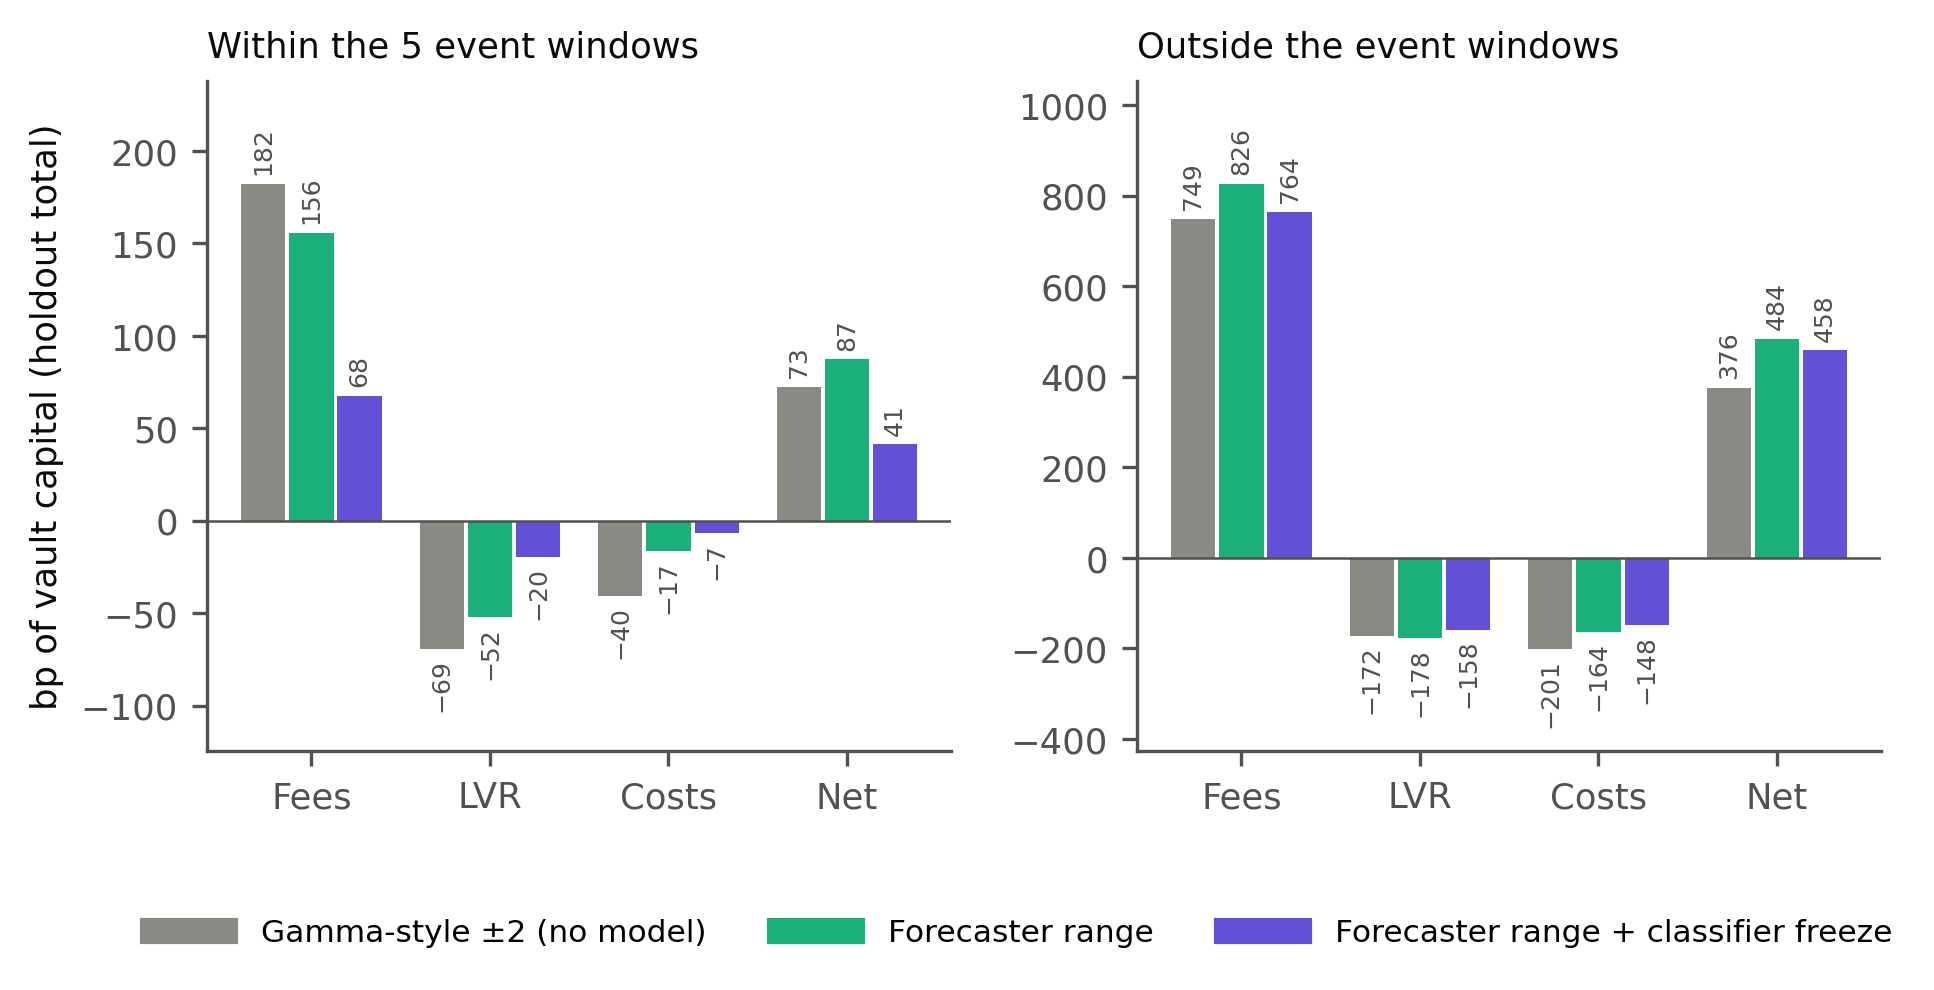
\includegraphics[width=\linewidth]{figures/lp_fees_lvr.png}
    \caption{Fee income, LVR, repositioning costs and net profit of the three vaults within the event windows
    (24 hours before to 48 hours after each 15\,bp event) and outside them, summed over the holdout (bp of the
    vault's capital).
    \href{https://github.com/QuantLet/onchain-insights/tree/main/14.\%20LP\%20vault\%20backtest}{\includegraphics[height=0.6\baselineskip]{figures/Quantlet LOGO.png}}}
    \label{fig:lp_fees_lvr}
\end{figure}

\paragraph{The classifier protects against depegs.} Pausing the forecaster vault during the classifier's
alerts cuts its LVR within the event windows by \lpFcKEvLVRCut\% (from \lpFcEvLVR{} to \lpFcKEvLVR\,bp),
its event drawdown by \lpFcKEventDDCut\% (from \lpFcEventDD{} to \lpFcKEventDD\,bp) and its maximum
drawdown by \lpFcKMaxDDCut\% (from \lpFcMaxDD{} to \lpFcKMaxDD\,bp). The Sharpe ratio rises from
\lpFcSharpe{} to \lpFcKSharpe. Relative to the Gamma-style vault, the two-model vault reduces the maximum
drawdown by \lpFcKvsGammaMaxDDCut\% and the event drawdown by \lpFcKvsGammaEventDDCut\%, and it has the
smallest maximum drawdown and the highest Sharpe ratio of all actively managed vaults that do not use
future information.
The pause has the same effect on the Gamma-style vault, whose event drawdown falls by \lpGKEventDDCut\%,
from \lpGammaEventDD{} to \lpGKEventDD\,bp.

These reductions come from the timing of the alerts, not from pausing as such. Randomly timed pauses with
the classifier's episodes rarely achieve comparable reductions: the placebo $p$-values are \lpPFcEventDD{} for the event
drawdown and \lpPFcMaxDD{} for the maximum drawdown of the forecaster vault, and \lpPGammaEventDD{} and
\lpPGammaMaxDD{} for the Gamma-style vault (Figure~\ref{fig:lp_placebo} in Appendix~\ref{sec:lp_appendix}).
Lead time distinguishes the classifier from the price trigger, which acts on the same events but only once
the threshold is breached. With the classifier, the event drawdown of the forecaster vault is
\lpFcKEventDD\,bp, against \lpFcPEventDD\,bp with the price trigger and \lpFcOEventDD\,bp with the 24-hour
oracle, and it is smaller than with the price trigger in \lpFcKBetterEvents{} of the \lpNEvents{} events
(Table~\ref{tab:lp_events}). The ordering holds with every forecaster (Table~\ref{tab:lp_forecasters}) and in
every cost, size and competition scenario (Table~\ref{tab:lp_sensitivity}).

\input{lp/tab_lp_events}

\paragraph{Why the pause lowers net profit.} The pause is insurance, and it has a premium: it lowers net
profit by \lpFcKCost\,bp per year for the forecaster vault and \lpGKCost\,bp for the Gamma-style vault,
against \lpFcPCost{} and \lpGPCost\,bp for the price trigger. Figure~\ref{fig:lp_fees_lvr} shows where the
premium comes from. In this pool, depeg periods bring very large trading volumes, so a vault that keeps
repositioning earns fees that exceed its LVR on average: within the event windows the forecaster vault earns
\lpFcEvFees\,bp of fees against \lpFcEvLVR\,bp of LVR. A paused vault drifts out of range and forgoes both;
its fee income in the event windows falls to \lpFcKEvFees\,bp. In addition, \lpFalseEpisodes{} of the
classifier's \lpEpisodes{} episodes are not followed by an event and pause the vault in calm periods.
Figure~\ref{fig:lp_event_zoom} illustrates both cases. On 3 February 2025 the pause stops the accumulation of
LVR but also of fees. On 4 February 2026 the alerts start the day before the breach, and the paused vault
avoids the LVR that the other vaults incur when the price spikes to \lpMaxDepeg\,bp. The holdout contains no
severe depeg, so over this sample the premium exceeds the losses it avoids, as for any insurance whose value
lies in the tail. When half of the fee income is captured by just-in-time liquidity, the paused vaults earn
more than those that keep repositioning (Table~\ref{tab:lp_sensitivity}).

\begin{figure}[pos=!htbp,align=\centering]
    \centering
    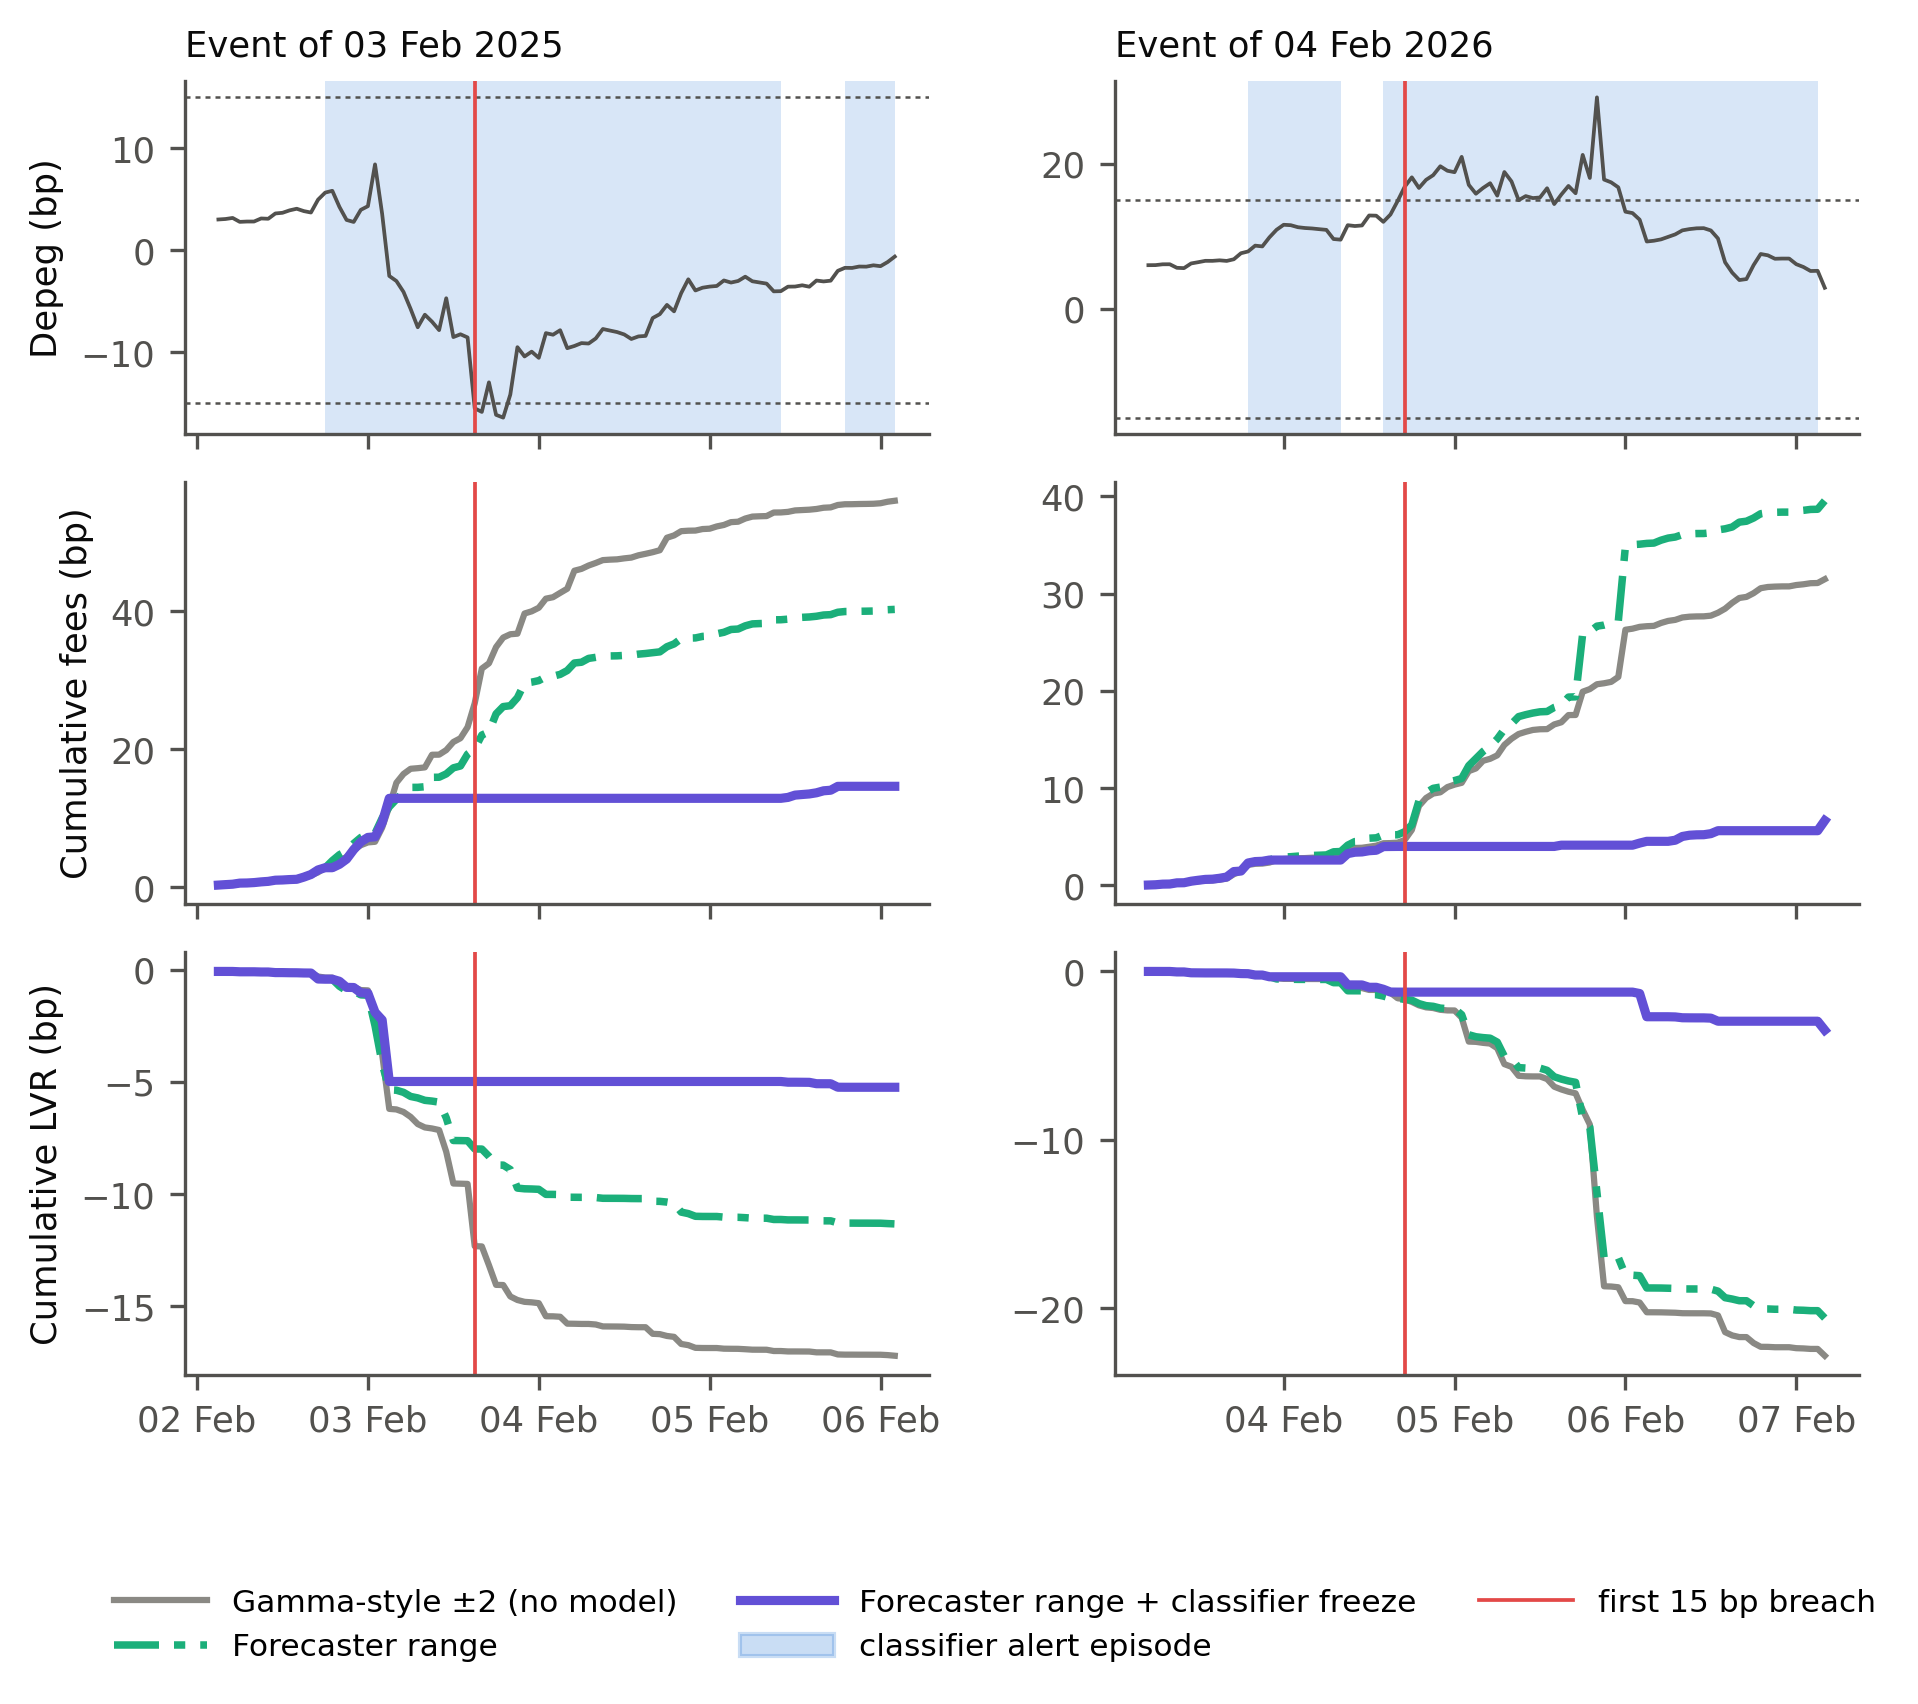
\includegraphics[width=\linewidth]{figures/lp_event_zoom.png}
    \caption{Two holdout events. Top: pool depeg and classifier alert episodes; the red line marks the first
    15\,bp breach. Middle and bottom: cumulative fee income and cumulative LVR from the start of the window.
    The paused vault gives up fees and avoids LVR.
    \href{https://github.com/QuantLet/onchain-insights/tree/main/14.\%20LP\%20vault\%20backtest}{\includegraphics[height=0.6\baselineskip]{figures/Quantlet LOGO.png}}}
    \label{fig:lp_event_zoom}
\end{figure}

\paragraph{Out-of-sample check.} In 2024 the classifier's out-of-fold alerts detected \lpYDetected{} of the
\lpYNEvents{} events in the sample, so the forecaster's protection matters more (Table~\ref{tab:lp_2024}).
The event drawdown is \lpYGammaEventDD\,bp for the Gamma-style vault, \lpYGKEventDD\,bp with the classifier's
pauses, \lpYFcEventDD\,bp with the forecaster range and \lpYFcKEventDD\,bp with both. In this sample the
15\,bp price trigger performs similarly to the classifier once ranges are sized by the forecaster
(\lpYFcPEventDD\,bp), while for the Gamma-style vault the classifier gives the smaller maximum drawdown
(\lpYGKMaxDD{} against \lpYGPMaxDD\,bp).

\paragraph{A severe depeg.} Table~\ref{tab:lp_stress} and Figure~\ref{fig:lp_stress} illustrate the tail
that the pause insures against, using the USDC depeg of March 2023, when the pool price fell by up to
\lpStressMinDepeg\,bp. Fees are not observed in this period and the classifier's out-of-fold alerts do not
cover it, so the scenario reports losses only and starts the pause at, or a fixed number of hours before,
the first 15\,bp breach. Vaults that keep repositioning lose 20--30\% of their capital: the Gamma-style vault
repositions \lpStressGammaRepo{} times and loses \lpStressGamma\,bp, and the forecaster vault loses
\lpStressFc\,bp. Pausing at the breach limits the loss to a few basis points (\lpStressGammaBreach\,bp for
the Gamma-style vault), and pausing \lpStressLead{} hours earlier reduces it further
(\lpStressGammaLead\,bp). In such a crash the decisive protection is to stop repositioning around the event;
lead time adds a few basis points. In the moderate events of the holdout, where much of the damage occurs
before the breach, lead time halves the losses.

\input{lp/tab_lp_stress}

\begin{figure}[pos=!htbp,align=\centering]
    \centering
    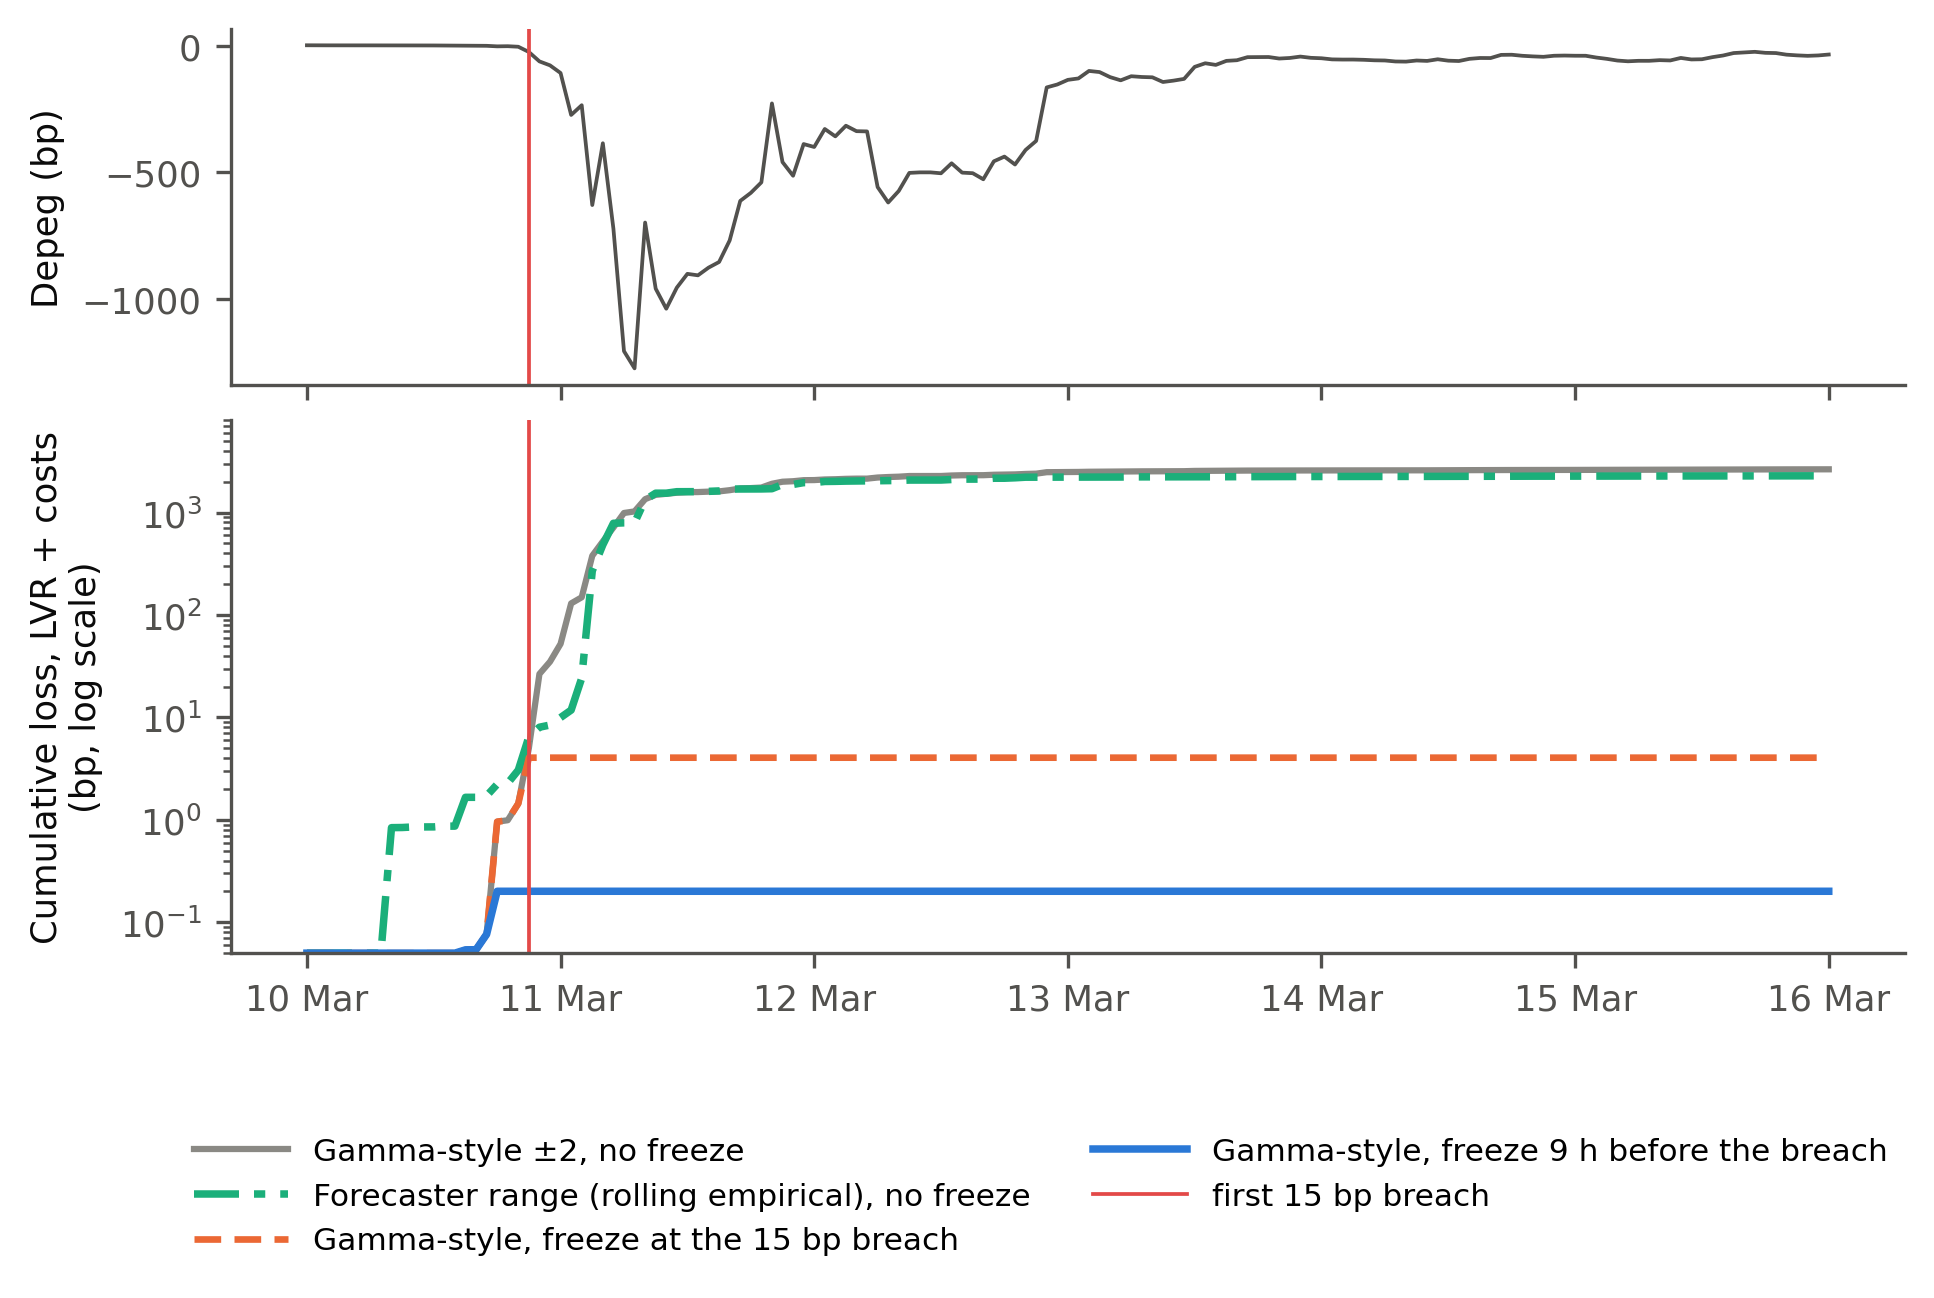
\includegraphics[width=\linewidth]{figures/lp_stress_march2023.png}
    \caption{USDC depeg of March 2023. Top: pool depeg; the red line marks the first 15\,bp breach. Bottom:
    cumulative losses from LVR and repositioning costs, on a logarithmic scale; fee income is not observed in
    this period.
    \href{https://github.com/QuantLet/onchain-insights/tree/main/14.\%20LP\%20vault\%20backtest}{\includegraphics[height=0.6\baselineskip]{figures/Quantlet LOGO.png}}}
    \label{fig:lp_stress}
\end{figure}


% -----------------------------------------------------------------------------------------------------
% [F1] CONCLUSION -- new paragraph after the second paragraph (ending
%      "... potential severity of prospective pool-price deviations.")
% -----------------------------------------------------------------------------------------------------
An economic evaluation supports these complementary roles. In a backtest of liquidity provision to the
monitored pool, the forecaster sizes the vault's range: its predictive intervals raise net profit and the
Sharpe ratio relative to a Gamma-style vault, and reduce repositioning costs and daily tail losses. The
classifier protects against depegs: pausing repositioning during its alerts cuts the losses to arbitrageurs
around the held-out events by \lpFcKEvLVRCut\% and the drawdowns within them by \lpFcKEventDDCut\%, more
than a price trigger at the same threshold, which shows that its lead time has economic value. Together,
the two models reduce the vault's maximum drawdown by \lpFcKvsGammaMaxDDCut\%, at the cost of part of the
high fee income of depeg periods. In the March 2023 USDC depeg, vaults that keep repositioning lose 20--30\%
of their capital, the tail risk against which such protection is designed.

% [F2] CONCLUSION -- add to the final (perspectives) paragraph, before its last sentence
The economic evaluation suggests further extensions: classifiers trained at the thresholds at which a given
position is managed, and decisions that are costly to reverse within the hour, such as unwinding large or
leveraged positions, where the lead time of the early-warning policy should be most valuable.


% -----------------------------------------------------------------------------------------------------
% [G] APPENDIX -- new section, e.g. before "\section{Data Appendix}"
% -----------------------------------------------------------------------------------------------------
\section{Liquidity-provision backtest: additional results}\label{sec:lp_appendix}

Table~\ref{tab:lp_forecasters} applies the range rule to every forecaster, with asymmetric intervals (the main
specification) and with symmetric ranges of the same width centred on the median forecast.
Table~\ref{tab:lp_2024} repeats the comparison on 2024, Table~\ref{tab:lp_sensitivity} varies costs, vault
size, competition from just-in-time liquidity and fee reinvestment, and Figure~\ref{fig:lp_placebo} shows the
placebo distributions.

\input{lp/tab_lp_forecasters}

\input{lp/tab_lp_2024}

\input{lp/tab_lp_sensitivity}

\begin{figure}[pos=!htbp,align=\centering]
    \centering
    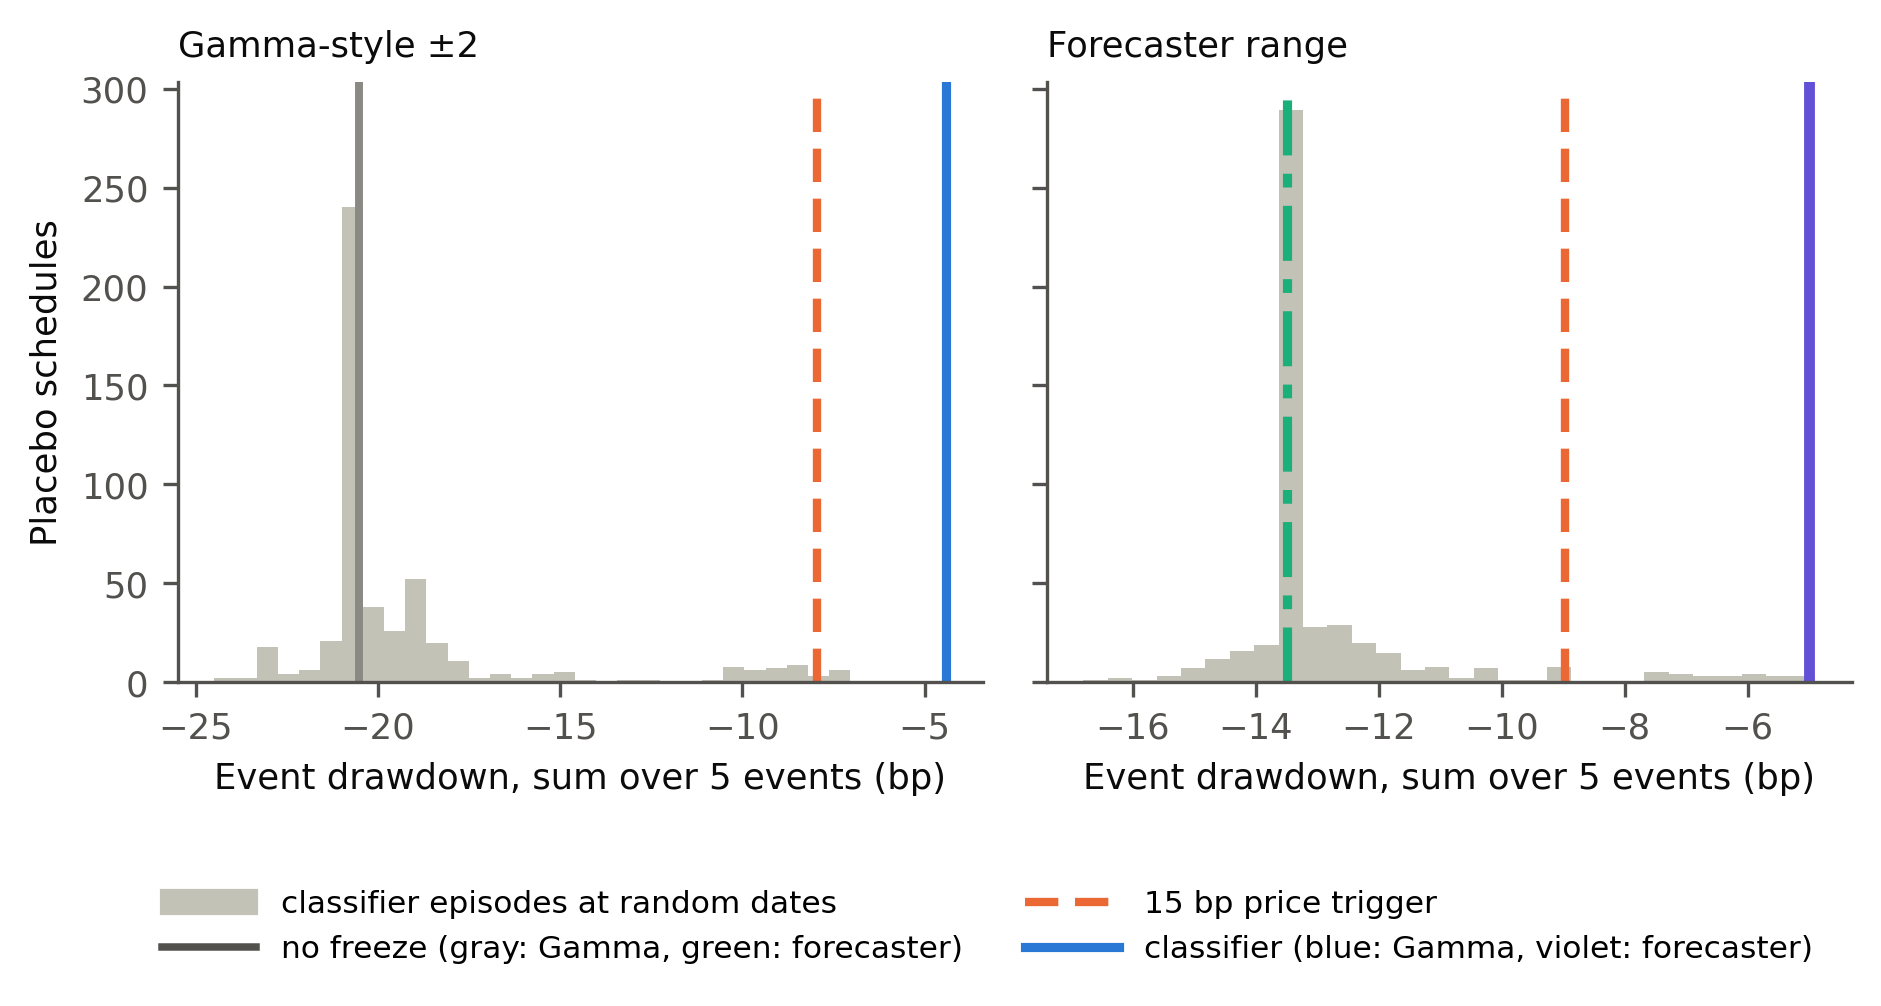
\includegraphics[width=\linewidth]{figures/lp_placebo.png}
    \caption{Event drawdown of the Gamma-style vault (left) and the forecaster vault (right) when the
    classifier's alert episodes are placed at random dates, compared with the vault without pauses, with the
    15\,bp price trigger, and with the classifier's alerts.
    \href{https://github.com/QuantLet/onchain-insights/tree/main/14.\%20LP\%20vault\%20backtest}{\includegraphics[height=0.6\baselineskip]{figures/Quantlet LOGO.png}}}
    \label{fig:lp_placebo}
\end{figure}
